\fenicschapter{Finite elements for incompressible fluids}
              {Finite elements for incompressible fluids}
              {Andy R. Terrel, L. Ridgway Scott, Matthew G. Knepley,
               Robert C. Kirby and Garth N. Wells}
              {terrel}


The structure of the finite element method offers a user a range of
choices.  This is especially true for solving incompressible fluid
problems, where theory points to a number of stable finite element
formulations. Using automation tools, we implement and examine various
stable formulations for the steady-state Stokes equations.  It is
demonstrated that the expressiveness of the FEniCS Project components
allows solvers for the Stokes problem that use various element
formulations to be created with ease.
%------------------------------------------------------------------------------
\section{Stokes equations}
\label{sec:terrel:Stokes}

The Stokes equations describe steady, incompressible low Reynolds number
flows. For a domain $\Omega \subset \mathbb{R}^{d}$, where $1 \le d \le 3$,
the Stokes equations read:
%
\begin{align}
     -\Delta u + \nabla p &= f \quad \mbox{in} \ \Omega,
\label{eqn:terrel:StrongStokes}
\\
      \nabla\cdot u &= 0 \quad \mbox{in} \ \Omega,
\label{eqn:terrel:StrongStokes_icomp}
\\
      u &= 0 \quad \mbox{on} \  \partial \Omega,
\end{align}
%
where $u : \Omega \rightarrow \mathbb{R}^{d}$ is the velocity field, $p
: \Omega \rightarrow \mathbb{R}$ is the pressure field and $f : \Omega
\rightarrow \mathbb{R}^{d}$ is a source term.

In developing a variational formulation for solving the Stokes equations,
a possibility is to search for solutions to a variational formulation of
\eqref{eqn:terrel:StrongStokes} in a space of divergence-free functions,
thereby satisfying \eqref{eqn:terrel:StrongStokes_icomp} by construction.
However, this does not translate well to finite element
formulations. Alternatively, a mixed variational formulation can be
considered as follows. Let $V = [H^{1}_{0}(\Omega)]^d$ and $\Pi = \{q \in
L^2(\Omega) : \int_\Omega q \dx = 0\}$.  Given $f \in [L^{2}(\Omega)]^d$,
find functions $u \in V$ and $p \in \Pi$ such that
%
\begin{align}
    a(u, v) + b(v, p)  &=  (f, v) \quad \forall \ v \in V,
\label{eqn:stokes_momentum}
\\
    b(u, q) &= 0 \quad \forall \ q \in \Pi,
\label{eqn:stokes_continuity}
\end{align}
%
where
%
\begin{align}
  a(u, v) &:= \int_\Omega \nabla{u} \cdot \nabla v \dx,
\\
  b(v, q) &:= \int_\Omega (\nabla\cdot v) \, q \dx.
\\
  (f, v) &:= \int_\Omega f \cdot v \dx.
\end{align}
%------------------------------------------------------------------------------
\section{Finite element formulations for the mixed Stokes problem}

We will consider in this section finite element formulations
for finding approximate solutions to the mixed formulation in
\eqref{eqn:stokes_momentum} and~\eqref{eqn:stokes_continuity}.  The Stokes
problem has been studied extensively in the context of finite element
methods, with some key results presented in \citet{BrezziFortin1991}
and \citet{BrennerScott2008}.  It is a challenging problem on a number
of fronts.  Firstly, finite element subspaces of $V$ and $\Pi$ must be
chosen carefully to ensure stability of the resulting finite element
problem. Secondly, the mixed variational form is a saddle point problem,
which leads to indefinite matrix equations. Such systems are particularly
taxing on iterative linear solvers.  Moreover, conservation of mass requires
that the velocity field is divergence-free; very few schemes can satisfy
this condition point-wise.  The degree to which this condition is imposed
depends on the specific scheme.

Stable mixed finite element methods for the Stokes equations must satisfy
the Ladyzhenskaya--\babuska--Brezzi (LBB) (or inf--sup) compatibility
condition (see~\citet{BrezziFortin1991} for more details).  The most
straightforward scheme -- equal-order continuous Lagrange finite element
spaces for both pressure and velocity components -- leads to an unstable
problem.  Additionally, mixed element formulations can exhibit a type of
``locking'', which in practice is sometimes remedied by using inexact
quadrature for the $b(v, q)$-type terms.  This has been recognized as
equivalent to modifying the pressure space.  Here we take the modern
perspective and work with velocity and pressure spaces that are known
to satisfy the LBB condition.

An approach to circumventing the difficulties associated with the
saddle-point nature of the Stokes problem is to modify the discrete
variational problem such that it no longer constitutes a saddle-point
problem. With appropriate modification of the discrete problem, the
relevant stability condition becomes the more easily satisfied coercivity
condition. Careful modification can lead to a discrete problem that does
not violate consistency.

Few numerical studies of the Stokes problem address more than one
finite element formulation. This can be attributed to the difficultly
in implementing a number of the known stable methods. With automated
code generation, solvers for a range of methods can be easily produced;
it is as simple as redefining the finite element spaces or modifying the
variational formulation.  In the remainder of this section we demonstrate
the construction of a variety stable finite element solvers for the
mixed form of the Stokes equations.

%------------------------------------------------------------------------------
\subsection{Formulations based on compatible function spaces}

We consider a number of LBB-stable formulations that are based on the
selection of compatible functions spaces for the velocity and pressure
fields.  The generic \ufl{} input for most of these formulations is shown in
Figure~\ref{code:terrel:var:mixed}.  Following the \ufl{} convention, the
bilinear and linear forms are named {\tt a} and {\tt L}, respectively.
Different finite element spaces are defined via the element type for
the velocity ({\tt V\_element}), the basis function order for the velocity
({\tt V\_order}), the element type for the pressure ({\tt P\_element}) and
the basis function order for the pressure ({\tt P\_order}). From the input
in Figure~\ref{code:terrel:var:mixed}, \ffc{} generates the problem-specific
code used in numerical simulations.
%
\begin{figure}
\begin{python}
# Define function spaces
V = VectorFunctionSpace(mesh, V_element, V_order)
Q = FunctionSpace(mesh, P_element, P_order)
W = V * Q

# Define test and trial functions
(v, q) = TestFunctions(W)
(u, p) = TrialFunctions(W)

# Define the variational problems
a = inner(grad(v), grad(u))*dx - div(v)*p*dx + q*div(u)*dx
L = inner(v, f)*dx
\end{python}
\caption{Generic \ufl{} input for the mixed Stokes problem.}
\label{code:terrel:var:mixed}
\end{figure}

One of the most widely used family of finite elements for Stokes
equations is the Taylor--Hood family~\citep{TaylorHood1973,Boffi1997}.
It consists of a continuous $P_k$ ($k\geq 2$) Lagrange element for the
velocity components and a continuous $P_{k-1}$ Lagrange element for the
pressure field (see Figure~\ref{fig:terrel:THElements} for the $k=3$
case). The order of the pressure convergence is lower than that for the
velocity.  For the \ufl{} extract in Figure~\ref{code:terrel:var:mixed},
the Taylor-Hood element corresponds to {\tt V\_element = Lagrange},
{\tt V\_order = k}, {\tt P\_element = Lagrange} and {\tt P\_order = k-1}.
%
\begin{figure}
  \center
  \subfloat[$P_3$ for $V$]{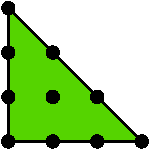
\includegraphics[width=0.4\textwidth]{chapters/kirby-6/pdf/P3.pdf}}
  \hspace{2em}
  \subfloat[$P_2$ for $\Pi$]{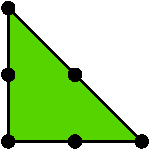
\includegraphics[width=0.4\textwidth]{chapters/kirby-6/pdf/P2.pdf}}
  \caption{A Taylor--Hood element with (a) cubic velocity basis and (b)
  quadratic pressure basis.}
\label{fig:terrel:THElements}
\end{figure}

The Crouzeix--Raviart element~\citep{CrouzeixRaviart1973} is a
non-conforming element that uses integral moments over cell
edges as a basis for the velocity, and a discontinuous pressure space
that is one order lower than the velocity space.  For the low-order case,
the velocity edge moments are equivalent to evaluating Lagrange basis
functions at the center of each edge and the pressure uses $P_0$
(see Figure~\ref{fig:terrel:CRElements}).  For the extract in
Figure~\ref{code:terrel:var:mixed},
the Crouzeix--Raviart element corresponds to
{\tt V\_element = CR}, {\tt V\_order = 1},
{\tt P\_element = DiscontinuousLagrange} and {\tt P\_order = 0}.
%
\begin{figure}
  \center
  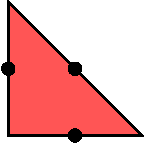
\includegraphics[width=0.4\textwidth]{chapters/kirby-6/pdf/CR1.pdf}
  \caption{Crouzeix--Raviart elements used for the velocity field.}
  \label{fig:terrel:CRElements}
\end{figure}

The MINI element~\citep{ArnoldBrezziFortin1984} enriches the velocity
space via bubble functions, $P_k + B_{k+3}$. The MINI element is
illustrated in Figure~\ref{fig:terrel:MINIElement}.  The pressure
space uses a continuous $P_{k}$ Lagrange element.  The MINI element
was proposed as a cheaper alternative to the Taylor--Hood element. The
MINI element is implemented using the ``element enrichment'' concept
from \ufl{}. The \ufl{} definition of the MINI function space is shown
in Figure~\ref{code:terrel:MINI}.  At the time of writing, it is only
implemented for $k=1, 2$.
%
\begin{figure}
  \center
  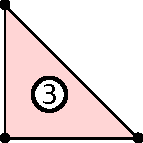
\includegraphics[width=0.4\textwidth]{chapters/terrel/pdf/MINI.pdf}
  \caption{Mini elements for velocity.  It enriches a $P_k$ element with
  a $k+3$ order bubble function.}
  \label{fig:terrel:MINIElement}
\end{figure}
%
\begin{figure}
\begin{python}
# Define function spaces
P = VectorFunctionSpace(mesh, "Lagrange", V_order)
B = VectorFunctionSpace(mesh, "Bubble", V_order + 2)
V = P + B
\end{python}
\caption{\ufl{} input for defining the MINI element.}
\label{code:terrel:MINI}
\end{figure}

Another possibility is to use a high-degree continuous Lagrange finite
element basis for the velocity components and a discontinuous element
that is two orders lower for the pressure field. We loosely call
this element ``CD'', for continuous velocity/discontinuous pressure.
\citet{BrezziFortin1991} discuss the $P_2-P_0$ case, and higher order
versions were analyzed in~\citet{MadayPateraRonquist1992}.  For the
low-order case, the CD method does not satisfy the LBB condition
and is commonly used with a stabilization parameter or enriched with
bubble functions. This case is not discussed here. For higher orders the
method is stable.  For the extract
in Figure~\ref{code:terrel:var:mixed}, the CD element corresponds to
{\tt V\_element = Lagrange}, {\tt V\_order = k}, {\tt P\_element =
DiscontinuousLagrange} and {\tt P\_order = k-2}.

\begin{table}
\centering
\caption{Element variables defining the different mixed methods.}
\label{tab:terrel:element_vars}
\medskip
\small
\begin{tabular}{|lccc|}
\hline
& Crouzeix--Raviart &  STAB & MINI \\
\hline
{\tt V\_element } & {\tt "CR"} &  {\tt "Lagrange"} & {\tt
 "MINI"}\\
{\tt V\_order} & $1$ & $k$ & $k$ \\
{\tt P\_element } & {\tt "Discontinuous Lagrange"} &  {\tt "Lagrange"} & {\tt "Lagrange"} \\
{\tt P\_order} & $0$ & $k$ & $k$ \\
{\tt stabilized } & {\tt False} & {\tt True} & {\tt False} \\
\hline
\hline
& CD &  Taylor--Hood &\\
\hline
{\tt V\_element } & {\tt
 "Lagrange"} & {\tt "Lagrange"} &\\
{\tt V\_order} & $k$ & $k$ &\\
{\tt P\_element } & {\tt "Discontinuous Lagrange"} & {\tt "Lagrange"} &\\
{\tt P\_order} & $k-2$ & $k-1$ &\\
{\tt stabilized } &  {\tt False} & {\tt False} &\\
\hline
\end{tabular}
\end{table}

Table~\ref{tab:terrel:element_vars} summarizes the specific variables
that appear the in the \ufl code in Figure~\ref{code:terrel:var:mixed}
for the different presented methods.

%------------------------------------------------------------------------------
\subsection{Pressure stabilized method}

To alleviate the difficulties of finding LBB-compatible function spaces,
one may use stabilization techniques.  Pressure stabilization converts the
finite-dimensional formulation from a saddle point problem to a coercive
problem. It is usually desirable to modify the finite-dimensional problem
such that consistency is not violated, which is the case if stabilisation
terms depend on the equation residual. For a more complete discussion
see~\citet{DoneaHuerta2003}.  The pressure stabilized method that we
consider involves:
%
\begin{align}
  a(u, v) + b(v, p)
      &=  (f, v) \quad \forall \ v \in V_{h},
\\
  b(u, q) +  (\delta\nabla{q},\nabla{p}) &=   (f, \delta \nabla q)
\quad \forall \ q \in \Pi_{h},
\end{align}
%
where $\delta$ is a stabilization parameter, and $V_{h} \subset V$
and $\Pi_{h} \subset \Pi$ are suitable finite element spaces. For
our tests, $\delta = 0.2 h_{K}^{2}$, where $h_{K}$ is two times
the circumference of the cell~$K$.
For the stabilised tests,
continuous Lagrange elements of the same order for both the pressure
and velocity spaces are used. This method will be referred to
as ``STAB''. The stabilized method that we adopt is simple, but it
does violate consistency for orders~$k > 1$.
Figure~\ref{code:terrel:var:stab} illustrates the
addition of the stabilization terms to the standard weak form in
Figure~\ref{code:terrel:var:mixed}.  Figure~\ref{tab:terrel:element_vars}
includes the definitions for the STAB element.

\begin{figure}
\begin{python}
# Sample parameters for pressure stabilization
h = CellSize(mesh)
beta = 0.2
delta = beta*h**2

# The additional pressure stabilization terms
a += delta*inner(grad(q), grad(p))*dx
L += delta*inner(grad(q), f)*dx
\end{python}
\caption{\ufl{} code to add stabilization to the mixed method
code in Figure~\ref{code:terrel:var:mixed}.}
\label{code:terrel:var:stab}
\end{figure}
%------------------------------------------------------------------------------
\section{A penalty approach: the Scott--Vogelius method}

Other solutions to deal with the LBB condition include the Uzawa
iteration method and penalty methods.  A combination of these two
approaches results in the iterated penalty method presented in
\citet{ScottVogelius1985}. Let $r \in \R$ and $\rho \in \R^{+}$ be
prescribed parameters, and we wish to find $u^n \in V_{h}$ such that
\begin{equation}
\label{eqn:terrel:IPStokes}
 a(u^n, v) + r(\nabla \cdot u^n, \nabla \cdot v)
      =  (f, v) - (\nabla\cdot v, \nabla \cdot w^n) \quad \forall \ v \in V_{h},
\end{equation}
%
where
%
\begin{equation}
\label{eqn:terrel:IPStokes_update}
   w^{n+1} = w^n + \rho u^n.
\end{equation}
%
The pressure may be recovered from the auxiliary field $w$ via $p =
\nabla\cdot w - C$, where $C$ is an arbitrary constant (since the
pressure field is only determined up to an arbitrary constant).
When computing the error in $p$, we subtract the average of $\nabla
\cdot w$ to account for~$C$. The algorithm initially assumes $w^0 =
0$, and then solves~\eqref{eqn:terrel:IPStokes} and updates $w$ via
\eqref{eqn:terrel:IPStokes_update}. The process is repeated until
$\|u^{n+1} - u^{n}\| < \epsilon$, where $\epsilon$ is a prescribed
tolerance. This method involves only one function space, but it
requires a higher-order continuous element ($k \ge 4$) and it solves the
divergence-free criteria exactly.  The iteration count and accuracy is
dependent upon the penalty parameters $\rho$ and~$r$.  For our experiments
we use $\rho = -r = 1 \times 10^{3}$.  The implementation of this form
is presented in Figure~\ref{code:terrel:var:ip}.
%
\begin{figure}
\begin{python}
# Define function space
V = VectorFunctionSpace(mesh, "Lagrange", V_order)

# Define test and trial functions
v = TestFunction(V)
u = TrialFunction(V)

# Define auxiliary function and parameters
w = Function(V);
rho = 1.0e3
r = -rho

# Define the variational problem
a = inner(grad(v), grad(u))*dx + r*div(v)*div(u)*dx
L = inner(v, f)*dx + inner(div(v), div(w))*dx
pde = VariationalProblem(a, L, bc0)

# Iterate to fix point
iters = 0; max_iters = 100; U_m_u = 1
while iters < max_iters and U_m_u > 1e-8:
    U = pde.solve()
    w.vector().axpy(rho, U.vector())
    if iters != 0:
        U_m_u = (U.vector() - u_old_vec).norm('l2')
    u_old_vec = U.vector().copy()
    iters += 1
\end{python}
\caption{\dolfin{} code for defining the Scott--Vogelius method.}
\label{code:terrel:var:ip}
\end{figure}

%------------------------------------------------------------------------------
\section{Numerical tests}
\label{sec:terrel:Results}

To evaluate the presented methods, we will compare the computed
results to a manufactured solution for different mesh refinements
and element orders. We also consider the lid driven cavity problem.
All simulations used \fenics{} tools to generate the discrete
problems (\ffc{} v0.7.0, \dolfin{} v0.9.4, \ufl{} v0.4.0, \ufc{}
v1.2.0), with the \packagefont{UMFPACK} LU solver (from the
\packagefont{SuiteSparse} package v3.4).  For iterative methods
applied to Stokes problems, we refer to Chapter~\ref{chap:mardal-4}
and \citet{ElmanSilvesterWathen2005}.  The number of the degrees of
freedom as a function of mesh size and element type for the considered
cases are shown in Table~\ref{tab:terrel:DOFs}.

\begin{figure}
\center
\subfloat[Unit square mesh $16 \times 16$ with cross pattern.]{
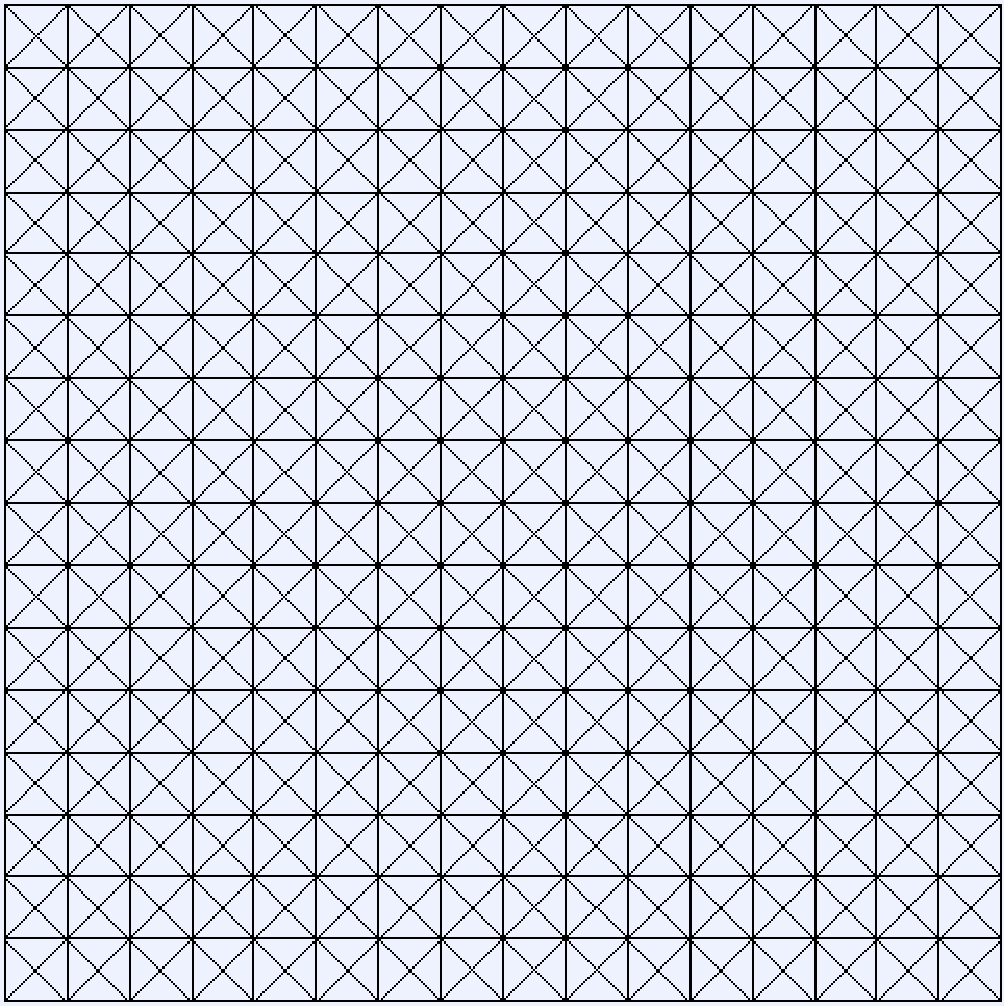
\includegraphics[width=0.4\textwidth]{chapters/terrel/pdf/mesh.pdf}
\label{fig:terrel:mesh}
}
\qquad
\subfloat[Velocity magnitude of test problem.]{
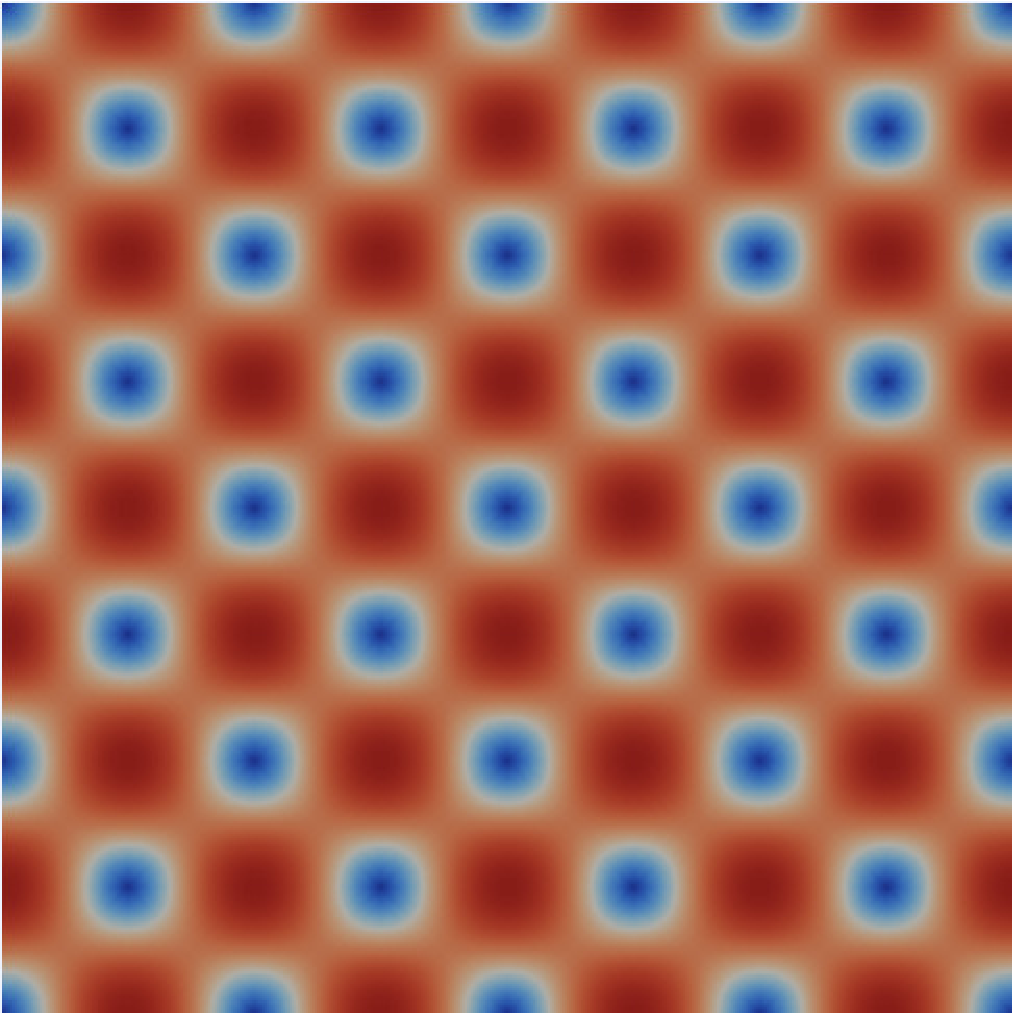
\includegraphics[width=0.4\textwidth]{chapters/terrel/pdf/vel_test.pdf}
\label{fig:terrel:vel_test}
}
\qquad
\subfloat[Velocity magnitude of lid driven cavity with streamlines.]{
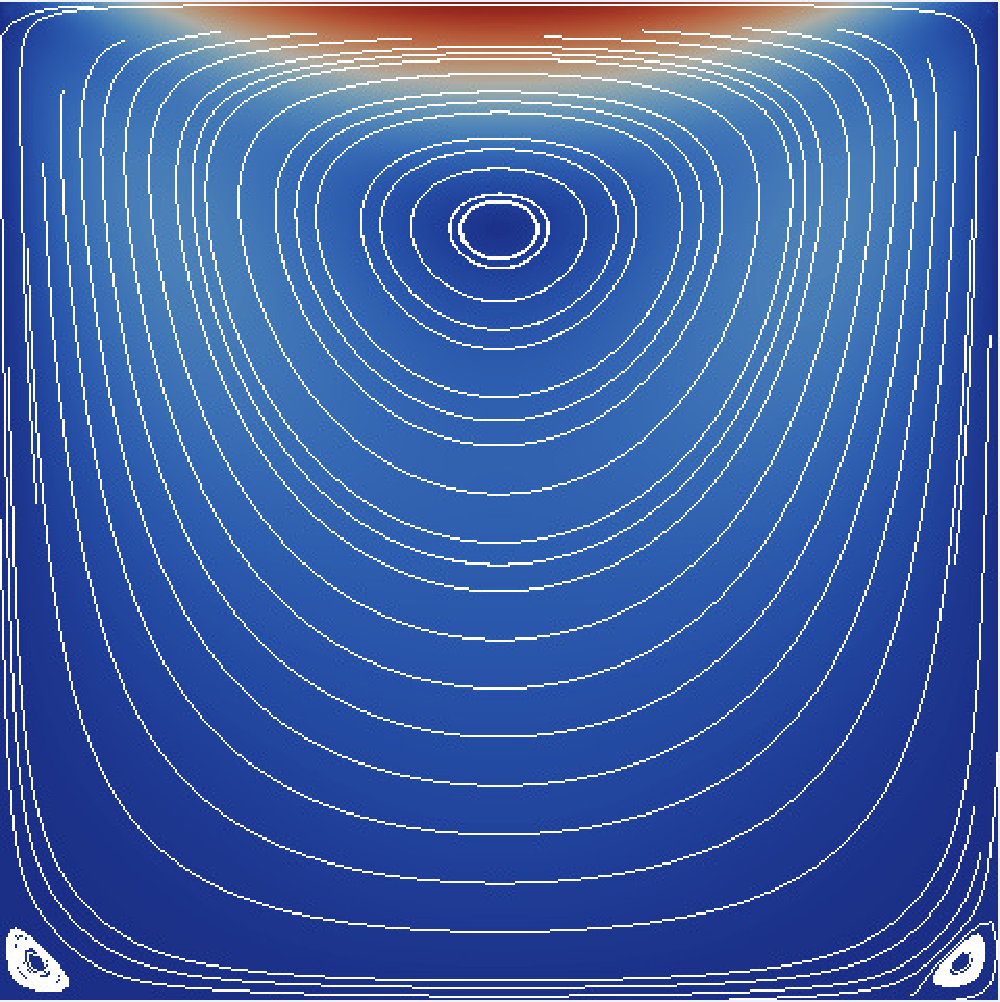
\includegraphics[width=0.4\textwidth]{chapters/terrel/pdf/vel_lid.pdf}
\label{fig:terrel:vel_lid}
}
\caption{Test mesh and solution plots.}
\label{fig:terrel:meshsolution}
\end{figure}

\begin{table}
  \center
  \medskip
  \small
  \begin{tabular}{|cc|rrr|}
    \hline
    k & n & Crouzeix--Raviart &  STAB & MINI \\
    \hline
    1&  8 &   1056 &   435 & 947  \\
      & 16 &   4160 & 1635 & 3683 \\
      & 32 & 16512 & 6339 & 14531 \\
    \hline
    2 &  8 & - &     1635 & 3171 \\
       & 16 & - &    6339 &  12483 \\
       & 32 & - &  24963 & 49539 \\
    \hline
    3 &  8 & - &    3603 & x \\
       & 16 & - & 14115 & x \\
       & 32 & - & 55875 & x \\
    \hline
    4 &  8 & - &    6339 & x \\
       & 16 & - & 24963 & x \\
       & 32 & - & 99075 & x \\
    \hline
    5 &  8 & - &      9843 &  x \\
       & 16 & - &   38883 &  x \\
       & 32 & - & 154563 & x \\
    \hline
    \hline
    k & n & CD & Taylor--Hood & Scott--Vogelius \\
    \hline
    2 &  8 &  1346 &   1235 & - \\
       & 16 &  5250 &   4771 & - \\
       & 32 & 20738& 18755 & - \\
    \hline
    3 &  8 &   3170 &   2947 & - \\
       & 16 & 12482 & 11523 & - \\
       & 32 & 49538 & 45571 & - \\
    \hline
    4 &  8 &   5762 &    5427 &   4226 \\
       & 16 & 22786 &  21347 & 16642 \\
       & 32 & 90626 &  84675 & 66050 \\
    \hline
    5 &  8 &      5762 &     8675 &     6562 \\
       & 16 &   36162 &   34243 &   25922 \\
       & 32 & 144002 & 136067 & 103042 \\
    \hline
\end{tabular}
  \caption{A comparison of the number of degrees of freedom for problem,
  organized by velocity order ($k$) and number of mesh divisions
  per dimension ($n$). A `-' indicates that the order for that particular
  element is not stable, undefined; a `x' indicates it is currently
  not implemented.}
  \label{tab:terrel:DOFs}
\end{table}

%------------------------------------------------------------------------------
\subsection{Simulation set-up}

For our tests, we use an $n \times n$ unit square mesh with a cross
pattern, as illustrated in Figure~\ref{fig:terrel:meshsolution}(a),
and use the following analytical solution:
%
\begin{align}
\label{eqn:terrel:testcase}
  f &=
    \begin{bmatrix}
      28\pi^2\sin(4\pi x)\cos(4\pi y)
      \\
      -36\pi^2\cos(4\pi x)\sin(4\pi y)
    \end{bmatrix},
\\
  u &=
  \begin{bmatrix}
    \sin(4\pi x)\cos(4\pi y)
      \\
     -\cos(4\pi x)\sin(4\pi y)
   \end{bmatrix},
\\
  p &= \pi\cos(4\pi x)\cos(4\pi y).
\end{align}
%
We consider a lid driven cavity problem with a quadratic
driving function on the top (see Figures~\ref{fig:terrel:meshsolution}(b)
and~\ref{fig:terrel:meshsolution}(c)).

Figures~\ref{code:terrel:domain:test} and~\ref{code:terrel:domain:lid}
show the \dolfin{} Python input for the considered problems.  To change
from the analytical test problem to the lid driven cavity, only a
change in the boundary condition functions and the right-hand side
$f$ are required.  The pressure field, which is determined only up to
an arbitrary constant, is ``pinned'' at zero at one pressure degree
of freedom.  Given one of the above domains and one of the defined
variational problems, \dolfin{} will use \ffc{} and \fiat{} to generate
the necessary computer code automatically, allowing for one script to
test all the methods.

\begin{figure}
\small
\begin{python}
# Define the boundary domains
class NoSlipDomain(SubDomain):
    def inside(self, x, on_boundary):
        return on_boundary

class PinPoint(SubDomain):
    def inside(self, x, on_boundary):
        return x[0] < DOLFIN_EPS and x[1] < DOLFIN_EPS

# Define mesh
mesh = UnitSquare(h_num, h_num, "crossed")

# Instantiate the boundary conditions, set the
# velocity dof values to the exact solution, and
# pinpoint the pressure.
noslip_domain = NoSlipDomain()
noslip = Expression(("sin(4*pi*x[0])*cos(4*pi*x[1])",
               "-cos(4*pi*x[0])*sin(4*pi*x[1])"))
pinpoint = PinPoint()
pin_val = Expression("pi*cos(4*pi*x[0])*cos(4*pi*x[1])")
bc0 = DirichletBC(W.sub(0), noslip, noslip_domain)
bc1 = DirichletBC(W.sub(1), pin_val, pinpoint, "pointwise")
bc = [bc0, bc1]

# Define the RHS
f = Expression(("28*pi**2*sin(4*pi*x[0])"\
         "cos(4*pi*x[1])",
         "-36*pi**2*cos(4*pi*x[0])*sin(4*pi*x[1])"))

\end{python}
\caption{\dolfin{} code for defining the test domain.}
\label{code:terrel:domain:test}
\end{figure}

\begin{figure}
\small
\begin{python}
# Define the boundary domains
class NoSlipDomain(SubDomain):
    def inside(self, x, on_boundary):
        return on_boundary and x[1] < 1.0 - DOLFIN_EPS

class Top(SubDomain):
    def inside(self, x, on_boundary):
        return on_boundary and x[1] > 1.0 - DOLFIN_EPS

class PinPoint(SubDomain):
    def inside(self, x, on_boundary):
        return x[0] < DOLFIN_EPS and x[1] < DOLFIN_EPS

# Define mesh
mesh = UnitSquare(h_num, h_num, "crossed")

# Instantiate the boundary conditions
noslip_domain = NoSlipDomain()
noslip_val = Constant(mesh, (0.0, 0.0))
top_domain = Top()
top_val = Expression(("x[0]*(1.0 - x[0])", "0.0"))
pinpoint = PinPoint()
pin_val = Constant(mesh, 0.0)

# Define the RHS
f = Constant(mesh, (0.0, 0.0))
\end{python}
\caption{\dolfin{} code for defining the lid-driven cavity domain.}
\label{code:terrel:domain:lid}
\end{figure}

In computing the error for the analytical test cases in terms of function
norms, the exact solution is interpolated using 10th Lagrange
functions on cells. The code for computing the error is presented in
Figure~\ref{code:terrel:error}.

\begin{figure}
\begin{python}
# Define a high order approximation to the exact solution
u_ex = Expression(("sin(4*pi*x[0])*cos(4*pi*x[1])",
               "-cos(4*pi*x[0])*sin(4*pi*x[1])"),
               element=VectorElement("Lagrange", triangle, 10))
p_ex = Expression("pi*cos(4*pi*x[0])*cos(4*pi*x[1])",
               element=FiniteElement("Lagrange", triangle, 10))

# Define the L2 error norm
M_u = inner((u_ex - u),(u_ex - u))*dx
M_p = (p_ex - p)*(p_ex - p)*dx

# Compute the integral
u_err = assemble(M_u, mesh=mesh)
p_err = assemble(M_p, mesh=mesh)

# Compute L2 error of the divergence
M_div = div(u)*div(u)*dx
div_err = assemble(M_div, mesh=mesh)
\end{python}
\label{code:terrel:error}
\caption{\dolfin{} code for computing the error in the $L^{2}$ norm. The
exact solution is interpolated using 10th order Lagrange polynomials
on cells.}
\end{figure}
%------------------------------------------------------------------------------
\subsection{Results}

The observed convergence orders for each method in the $L^{2}$
norm of the velocity field, calculated from a series of
refined meshes with $n$ in $\{8, 16, 32, 64\}$, are presented in
Table~\ref{tab:terrel:vel_error}. The optimal rate is $k + 1$, which is
observed for all formulations except the CD element.  The CD element
loses one order of convergence due to poor pressure approximation and
failure to satisfy the LBB condition.

\begin{table}
  \caption{The computed exponential of the convergence rates of the
  velocity, i.e., $k$ in $O(h^k)$ where $h$ is the width of the mesh
  element. This error uses $L^2$ for the different elements with $k=p+1$
  being the optimal error rate with $p$ as the order of the velocity
  field.  Notice that the CD method, as theoretically expected, loses
  an order of convergence and the MINI element does not do well for the
  second order case. }
  \label{tab:terrel:vel_error}
  \begin{center}
  \small
  \begin{tabular}{|c|ccc|}
    \hline
    p  & Crouzeix--Raviart &  STAB &  MINI \\
\hline
   1 & $2.01\pm 1 \times 10^{-2}$ & $1.93\pm 6 \times 10^{-2}$ & $2.03\pm 6 \times 10^{-2}$ \\
   2 & -                          & $3.02\pm 2 \times 10^{-2}$ & $2.77\pm 5 \times 10^{-2}$ \\
   3 & -                          & $4.00\pm 1 \times 10^{-2}$ & - \\
   4 & -                          & $4.99\pm 4 \times 10^{-3}$ & - \\
   5 & -                          & $5.98\pm 1 \times 10^{-2}$ & -\\
    \hline
    \hline
    p  &  CD  & Taylor--Hood & Scott--Vogelius \\
\hline
   2 & $2.15 \pm 1 \times 10^{-1}$ & $3.02 \pm 2 \times 10^{-2}$ & -  \\
   3 & $3.11 \pm 2 \times 10^{-2}$ & $3.98 \pm 1 \times 10^{-2}$ & -  \\
   4 & $4.07 \pm 1 \times 10^{-2}$ & $4.99 \pm 1 \times 10^{-3}$ & $5.00 \pm 2 \times 10^{-3}$\\
   5 & $5.10 \pm 5 \times 10^{-2}$ & $5.97 \pm 1 \times 10^{-1}$ & $5.97 \pm 1 \times 10^{-1}$\\
    \hline
   \end{tabular}
  \end{center}
\end{table}

To further compare the methods, a number of error and performance measures
for the case of a fourth-order velocity space with a suitably chosen
pressure space are presented. The Crouzeix--Raviart and MINI elements
are only implemented for low-order bases. For the sake of comparison,
they are computed on a finer mesh that has a comparable number of
degrees-of-freedom to the fourth-order Taylor--Hood element.

Figure~\ref{fig:terrel:4th_Order:vel} compares the $L^{2}$ error in
the velocity for the different methods. The velocity approximation
appears to converge for all elements.  The $L^{2}$ error in the pressure
is shown in Figure~\ref{fig:terrel:4th_Order:press}.  Unpredictable
behaviour for the pressure is observed for the CD element, whereas
convergence for the pressure field is observed for the other methods.
The $L^{2}$ norm of the divergence of the velocity field is presented
in Figure~\ref{fig:terrel:4th_Order:div}.  The divergence error for
the Crouzeix--Raviart and Scott--Vogelius are zero to within machine
precision for all meshes, as predicted by theory. The divergence error
for the MINI element is considerably greater than that for the other methods.

\begin{figure}
  \center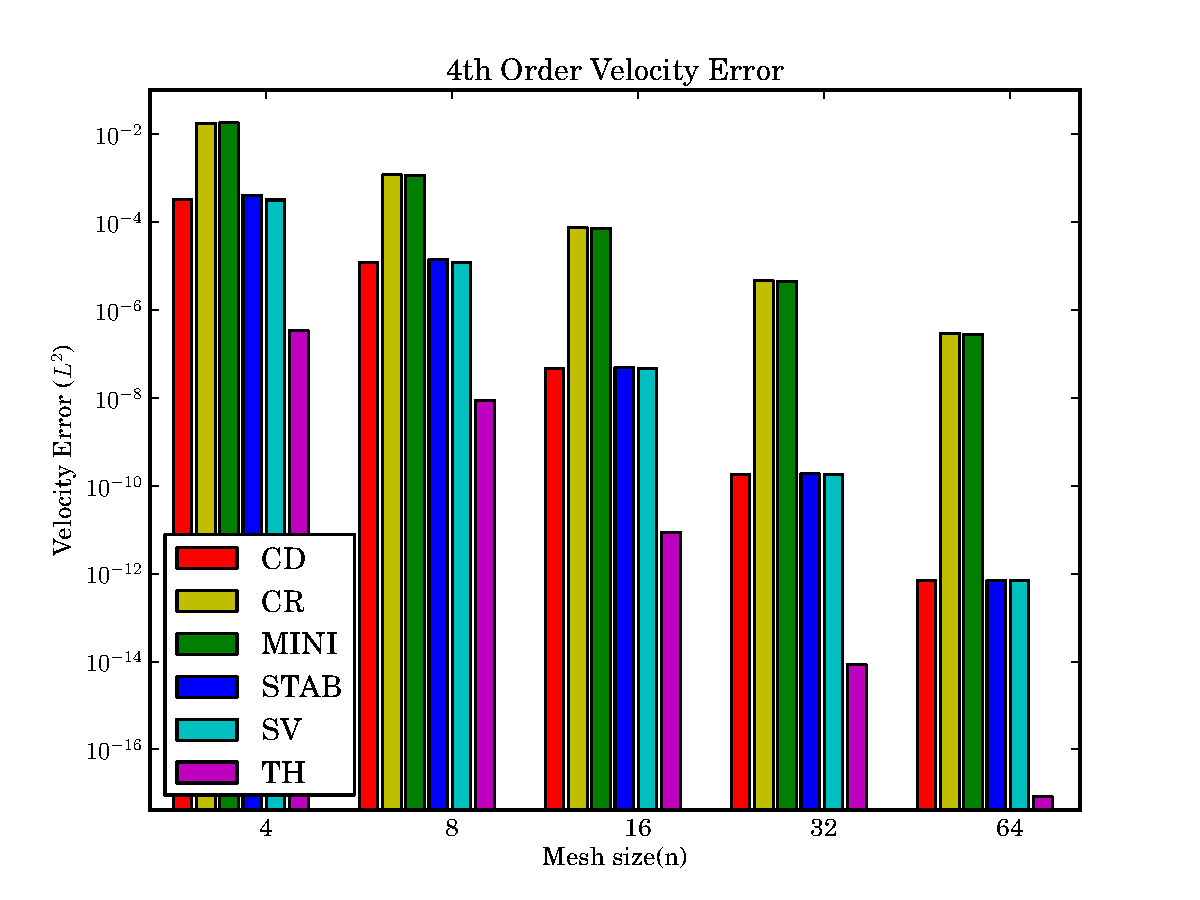
\includegraphics[width=\largefig]{chapters/terrel/pdf/vel_4.pdf}
  \caption{Velocity error of analytical test cases.}
    \label{fig:terrel:4th_Order:vel}
\end{figure}

\begin{figure}
  \center 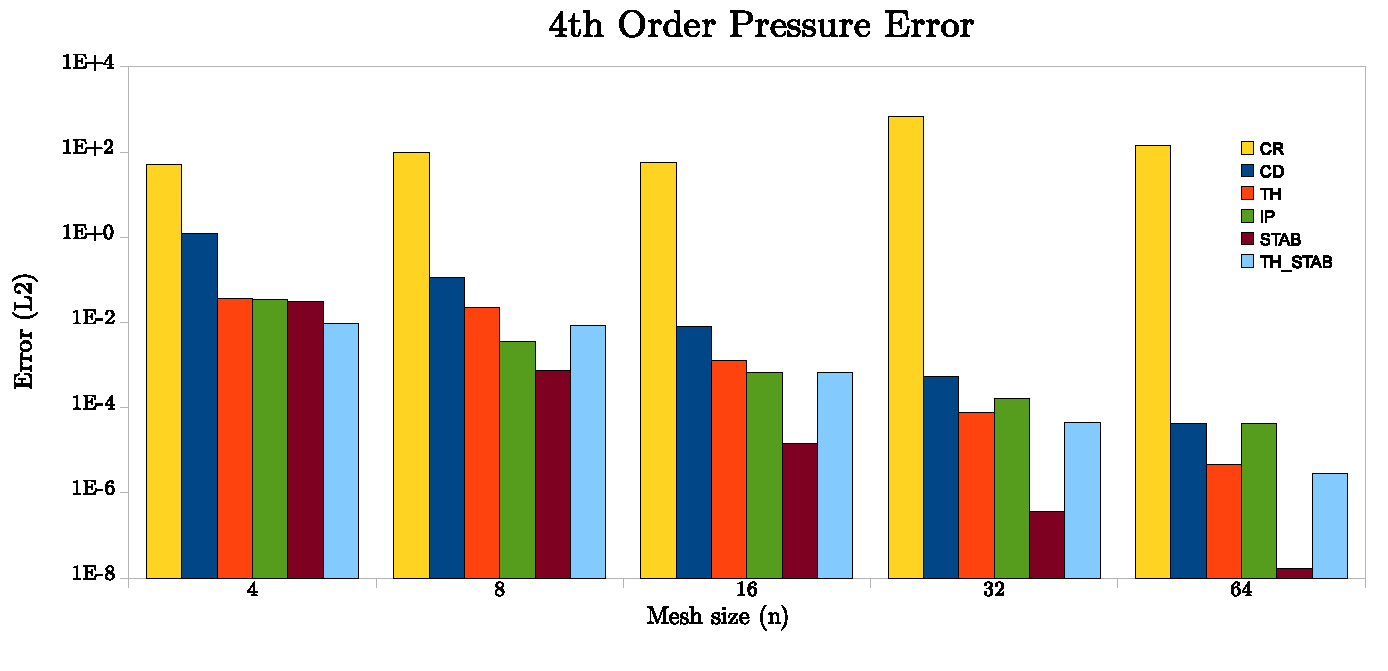
\includegraphics[width=\largefig]{chapters/terrel/pdf/press_4.pdf}
  \caption{Pressure error of analytical test cases.}
  \label{fig:terrel:4th_Order:press}
\end{figure}

\begin{figure}
  \center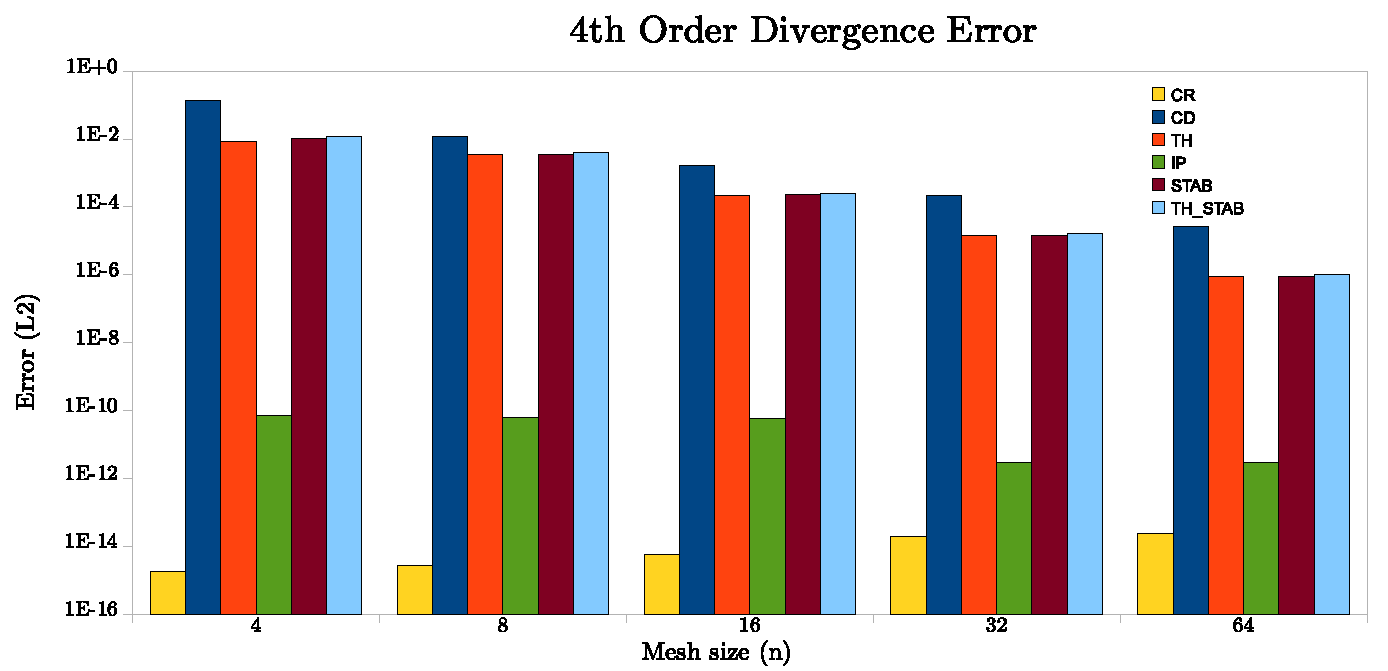
\includegraphics[width=\largefig]{chapters/terrel/pdf/div_4.pdf}
  \caption{Divergence error of analytical test cases.}
  \label{fig:terrel:4th_Order:div}
\end{figure}

Figure~\ref{fig:terrel:4th_Order:run} presents the run time for the
various fourth-order cases.  All run times, using a 2.6 GHz Intel Xeon,
measure the assembly and linear system solve time in the Python code. The
time required for the code generation is assumed to be negligible since
the generated code is cached and only affects the time for first run of a
simulation; our timings always come from the second run of the simulation.
Run times for the mixed elements scale with the the number of degrees of
freedom. The Scott--Vogelius method has better properties for iterative
solvers, hence it may be attractive for large-scale problems despite the
greater run time relative to other methods for the small problems tested.

\begin{figure}
  \center 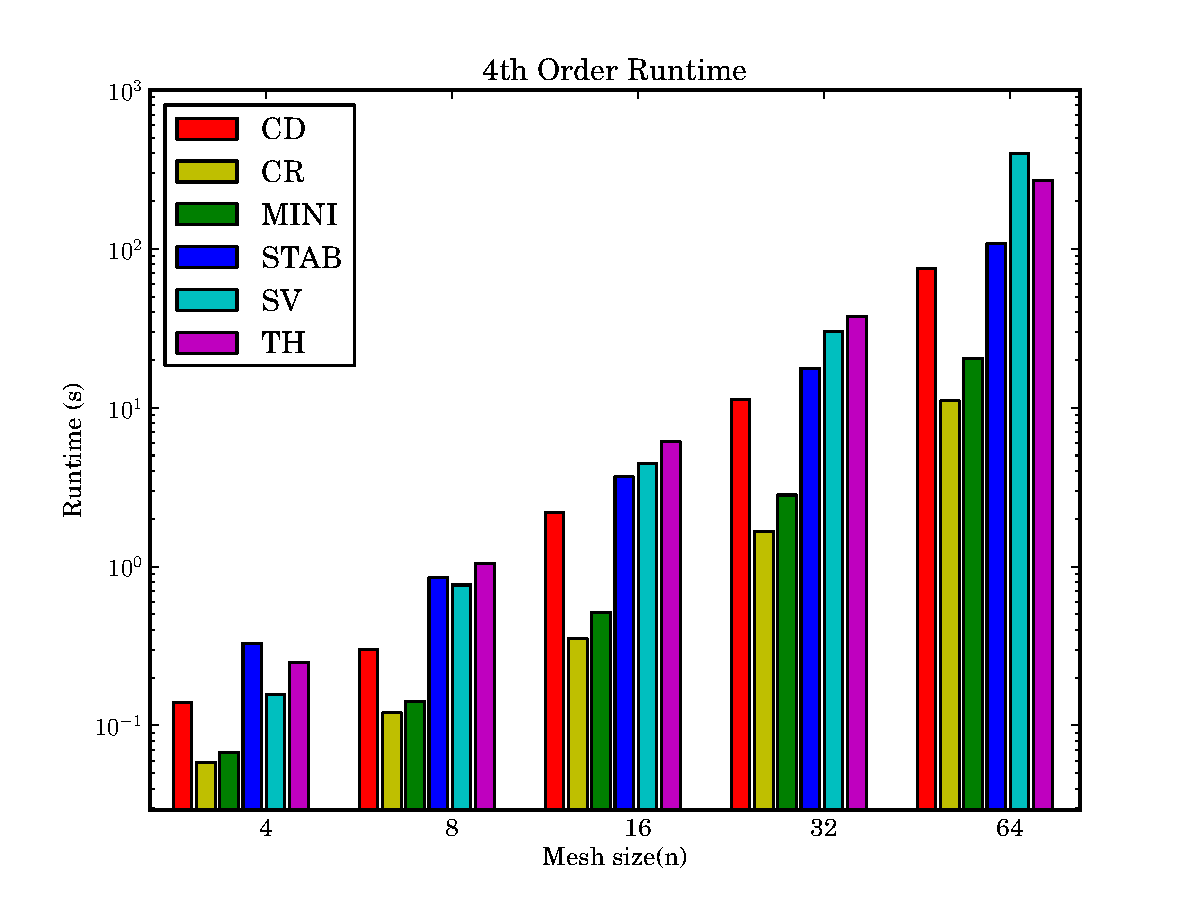
\includegraphics[width=\largefig]{chapters/terrel/pdf/run_4.pdf}
  \caption{Run times for the analytical test cases.  All velocity spaces,
    except Crouzeix--Raviart and MINI, are fourth-order and pressure
    spaces are determined by the method. Crouzeix--Raviart and MINI are
    computed on a finer mesh with a similar number of degrees-of-freedom
    to the fourth-order Taylor--Hood method. CR, TH, and SV refer to
    Crouzeix--Raviart, Taylor--Hood and Scott--Vogelius, respectively.}
  \label{fig:terrel:4th_Order:run}
\end{figure}

The $L^{2}$ norm of the divergence of the velocity for the lid driven
cavity problem is shown in Figure~\ref{fig:terrel:4th_Order_lid}.
Unlike for the already considered smooth test case, the divergence
error for the CD, MINI, stabilized and Taylor-Hood elements does not
decrease with mesh refinement.  A divergence error persists around
the pressure singularities at the corners of the lid, as is apparent
in Figure~\ref{fig:terrel:lid_div_error} for the Taylor-Hood case.
To solve the lid driven cavity problem with the Scott--Vogelius method,
the penalty parameter had to be increased to $1 \times 10^{8}$ for the
fixed point iteration to converge.

\begin{figure}
  \center 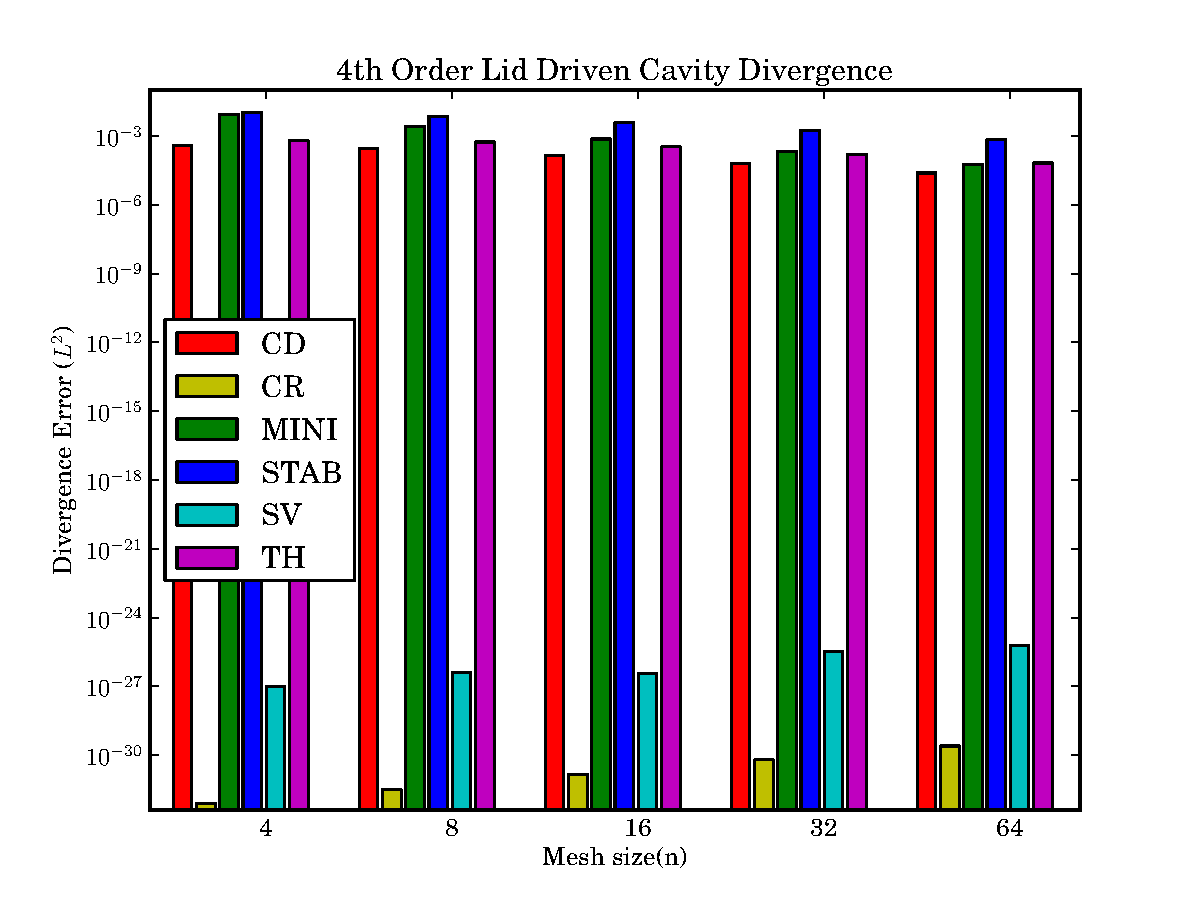
\includegraphics[width=\largefig]{chapters/terrel/pdf/div_4_test.pdf}
  \caption{Divergence error of the lid driven cavity.}
\label{fig:terrel:4th_Order_lid}
\end{figure}

\begin{figure}
  \center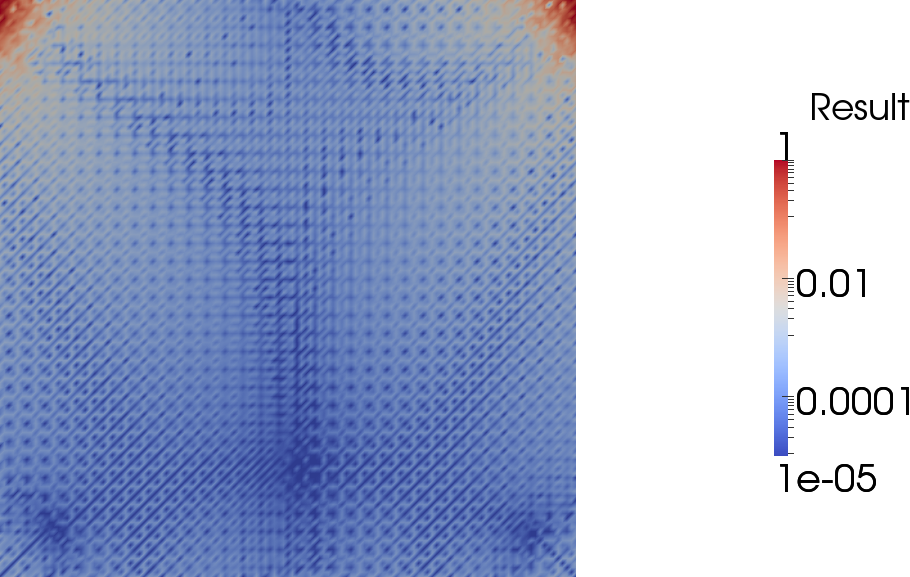
\includegraphics[width=0.8\textwidth]{chapters/terrel/png/lid_div_error.png}
  \caption{Global divergence error in lid driven cavity using $P_2$--$P_1$
  Taylor--Hood elements. Notice the corners of the lid produce error that is
  not local to the individual elements.}
  \label{fig:terrel:lid_div_error}
\end{figure}

%------------------------------------------------------------------------------
\section{Conclusions}

Comparisons between different finite elements for the Stokes problem have
been presented. The flexibility afforded by automated code generation
has been demonstrated via the ease with which a solvers for a range
of methods could be produced.
The observed convergence rates for all cases are consistent with \emph{a
priori} estimates.  Of the elements examined, the Crouzeix--Raviart
element and the Scott--Vogelius lead to the smallest divergence error.
If mass conservation properties are not crucial, the simplicity of
elements such as the Taylor--Hood or STAB is attractive.
%------------------------------------------------------------------------------
